\section{Auswertung}
In diesem Kapitel folgen nun die Messungen und Ergebnisse der drei Messaufgaben.

\begin{align}
	y = a \cdot exp \left( -ln(2) \cdot \frac{(x-x_0)^2}{dx^2} \right)
\label{form:gauss}
\end{align}

%gaussian-A
%\begin{align*}
%	\sqrt{\frac{ln(2)}{\pi}} \cdot \frac{a}{dx} \cdot exp \left(-ln(2) \cdot \frac{(x-x0)^2}{dx^2} \right)
%\end{align*}


\subsection{Photolumineszenz-Eigenschaften der kolloidalen Nanokristalle}
Die erste Aufgabe ist es, einige Eigenschaften der kolloidalen Nanokristalle anhand von Photoluminezsenzspektren zu untersuchen.
	\subsubsection{ Gr\"{o}{\ss}e der Nanokristalle}
Zun\"{a}chst soll die Gr\"{o}{\ss}e der kolloidalen Nanokristalle jeder Probe bestimmt werden.
Hierf\"{u}r wird jede einzelne Probe mit einem Laser der Wellenl\"{a}nge $405 \, nm$ angeregt und ein Photoluminezsenzspektrum (PL-Spektrum) von ca $320$ - $747 \, nm$ wird aufgenommen.
Diese PL-Spektren sind in Abbildung (\ref{abb:auf1a}) zu sehen. 
\begin{figure}[H]
\centering
	\begin{subfigure}[t]{0.4\textwidth}
	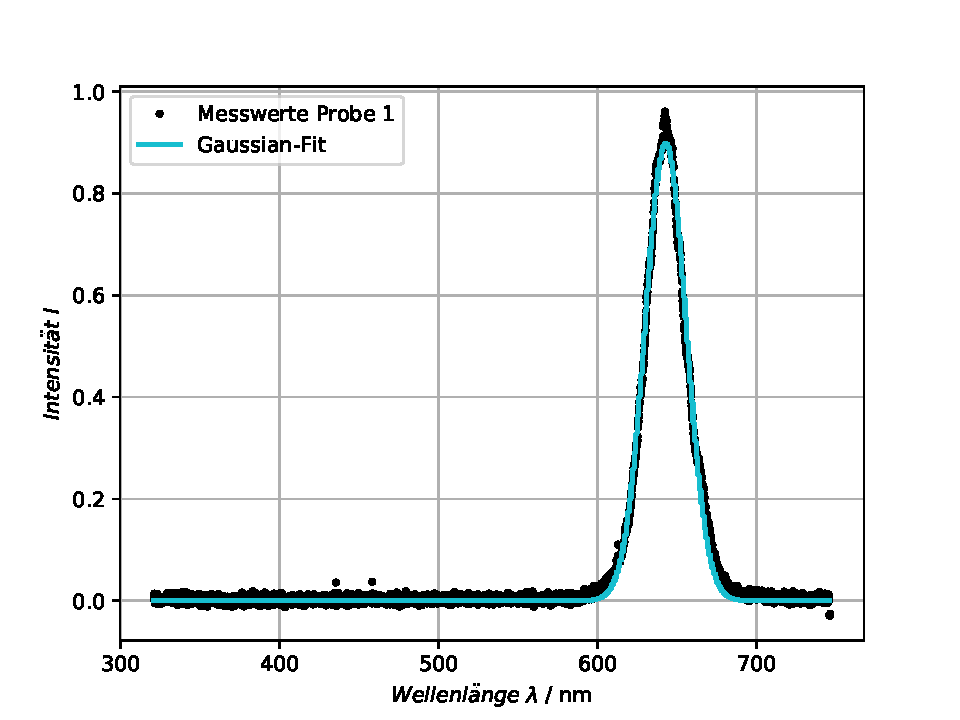
\includegraphics[width=\textwidth]{Plots/aufgabe1a_P1.pdf}
	\caption{Messung der Probe 1 mit Messdauer $1 \, s$.}
	\label{abb:A1_P1}
	\end{subfigure}
	~
	\begin{subfigure}[t]{0.4\textwidth}
	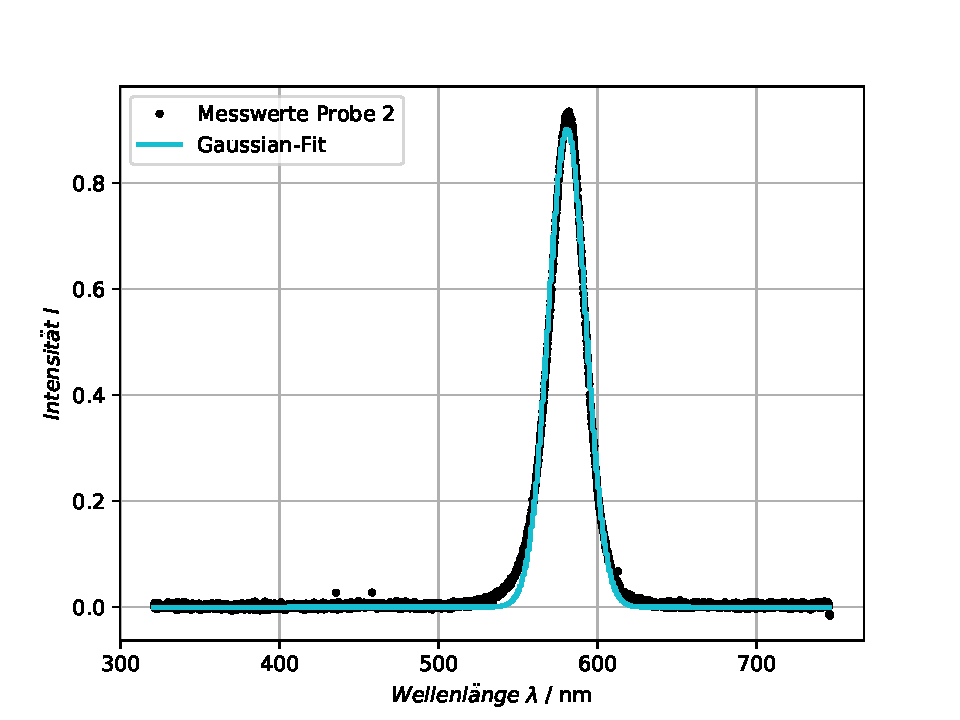
\includegraphics[width=\textwidth]{Plots/aufgabe1a_P2.pdf}
	\caption{Messung der Probe 2 mit Messdauer $0,5 \, s$.}
	\label{abb:A1_P2}
	\end{subfigure}
	~
	\begin{subfigure}[t]{0.4\textwidth}
	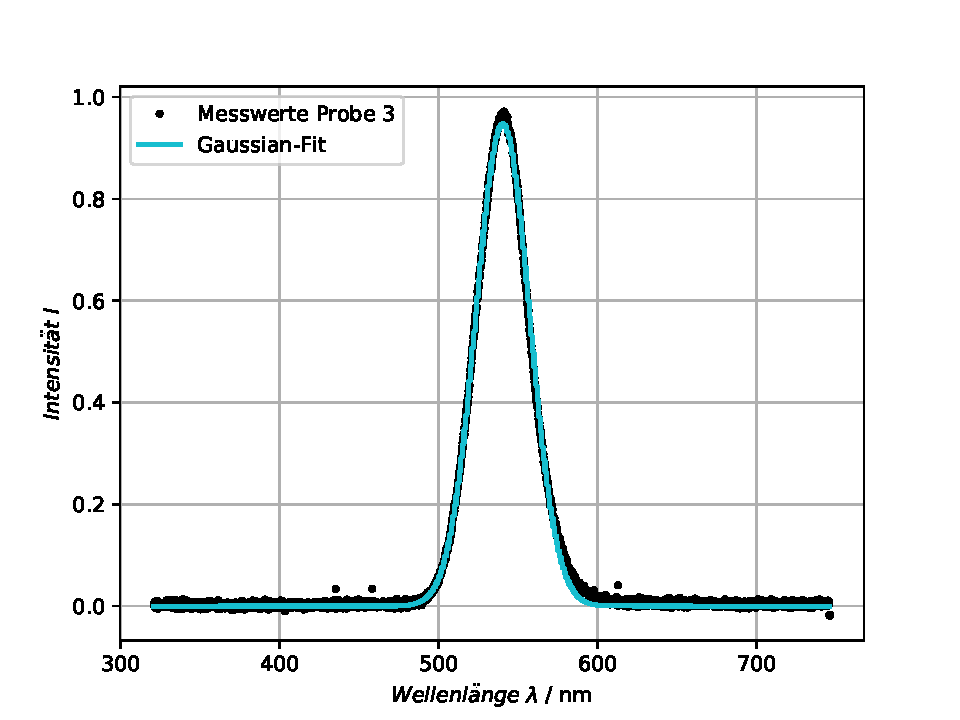
\includegraphics[width=\textwidth]{Plots/aufgabe1a_P3.pdf}
	\caption{Messung der Probe 3 mit Messdauer $0,65 \, s$.}
	\label{abb:A1_P3}
	\end{subfigure}
\caption{Photoluminessenzspektren der drei vorliegenden Proben mit einer Anregungswellenl\"{a}nge von 405 nm.}
\label{abb:auf1a}
\end{figure}
Alle drei Spektren weisen nur geringf\"{u}gige Abweichungen auf.
Mit Hilfe von Magicplots werden durch die Messwerte aller drei Pl-Spektren gau{\ss}f\"{o}rmige Ausgleichskurven gelegt.
Diese besitzen die in Formel (\ref{form:gauss}) beschriebene Form.
Die Variable $x_0$ gibt die Wellenl\"{a}nge der Probe an.
Mittels der Formeln (\ref{form:energie}) und (\ref{form:radius}) lassen sich nun die Gr\"{o}{\ss}e der Nanopartikel berechnen.
\begin{align}
	\Delta E_{r,i} &= h \frac{c}{\lambda_i} \label{form:energie}\\
	\Delta E_{r,i} &= E_g + \frac{h^2}{8r_{NP,i}} \left( \frac{1}{m_e^*} + \frac{1}{m_h^*} \right) \label{form:radius}
\end{align}
Alle Ergebnisse sind in Tabelle (\ref{tab:auf1a}) aufgelistet.
\begin{table}
	\centering
	\caption{Ergebnisse aus den Fit-Kurven der drei Messungen.}
\begin{tabular}{|r|cccc|}
	\hline
	{Probe} & \multicolumn{2}{c}{Wellenl\"{a}nge $\lambda$ / nm} & {Energie / eV} & {Radius $r_{NP}$ / nm} \\
	 & Theorie & experimentell &  &  \\
	\hline
	1	&	644	& 642,819 &	1,9289	&	7,717	\\
	2	&	580	& 580,832 &	2,1348	&	5,338	\\
	3	&	542	& 540,287 &	2,2949	&	4,502	\\
	\hline
\end{tabular}
\label{tab:auf1a}
\end{table}

	\subsubsection{Polarisation der Photolumineszenz}
Nachdem 
\begin{figure}[hbtp]
	\centering
	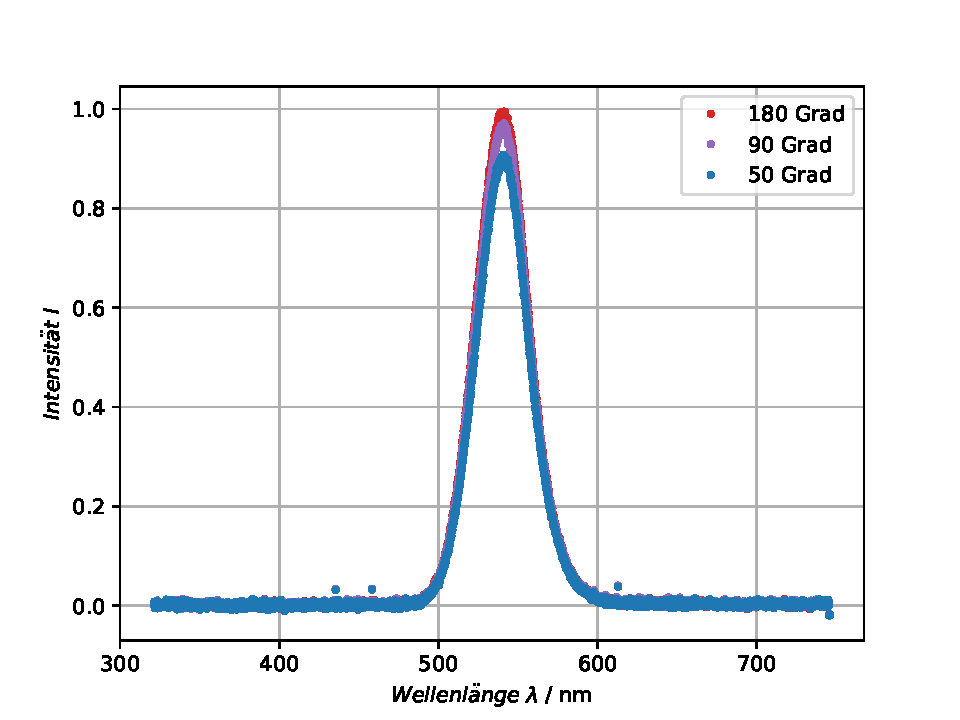
\includegraphics[width=0.5\textwidth]{Plots/aufgabe1b.pdf}
	\caption{PL-Spektrum der Probe 3 mit einer Anregungswellenl\"{a}nge von $405 \, nm$ f\"{u}r drei unterschiedliche Polarisationswinkel im Detektionspfad.}
	\label{abb:polarisation}
\end{figure}

	\subsubsection{Leistungsabh\"{a}ngige Peak-Energie}

\begin{figure}[H]
\centering
	\begin{subfigure}[t]{0.45\textwidth}
	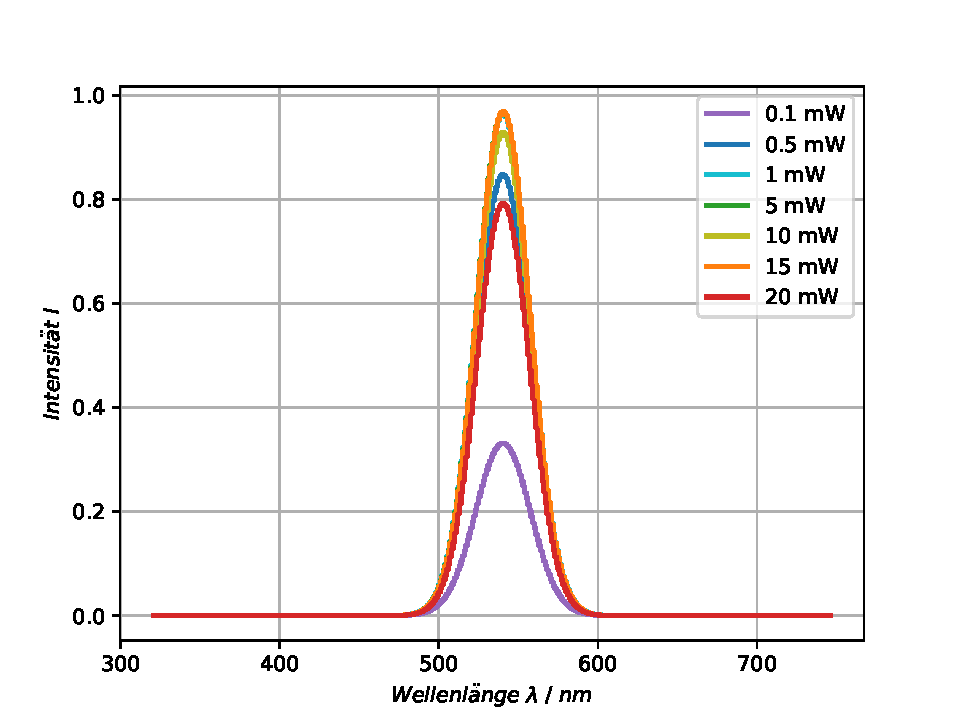
\includegraphics[width=\textwidth]{Plots/aufgabe1c2.pdf}
	\caption{Die aufgenommenen PL-Spektren f\"{u}r verschiedenen Laserleistungen.}
	\label{abb:verLeistung}
	\end{subfigure}
	~
	\begin{subfigure}[t]{0.45\textwidth}
	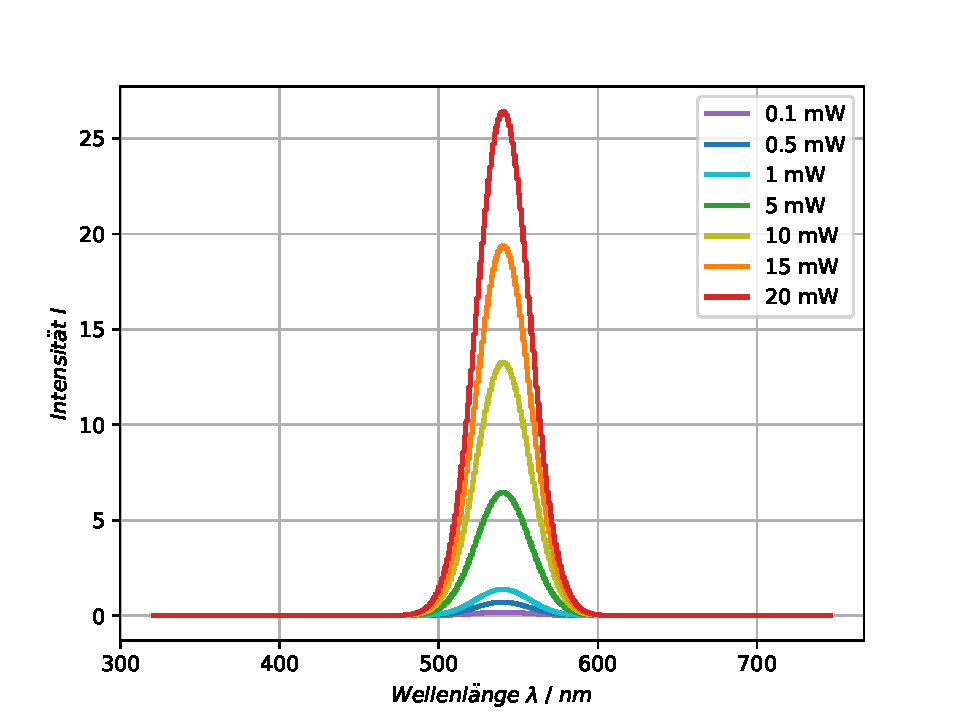
\includegraphics[width=\textwidth]{Plots/aufgabe1c2_1s.pdf}
	\caption{Die aufgenommenen PL-Spektren f\"{u}r verschiedenen Laserleistungen mit einer Messzeit von $1$ s.}
	\label{abb:verLeistung}
	\end{subfigure}
	~
	\begin{subfigure}[t]{0.45\textwidth}
	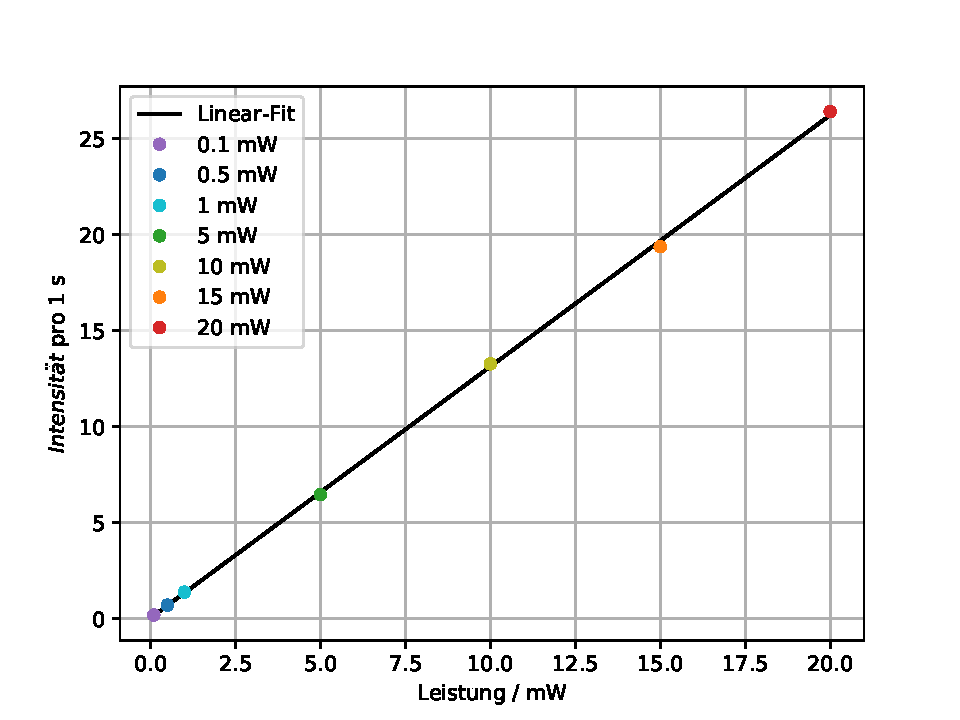
\includegraphics[width=\textwidth]{Plots/aufgabe1c3.pdf}
	\caption{Die Peak-Energien der PL-Spektren mit linearem Fit.}
	\label{abb:Leistungen_fit}
	\end{subfigure}
\caption{Messung der Peak-Energie der Probe 3 mit einer Anregungswellenl\"{a}nge von $405 \, nm$ f\"{u}r unterschiedliche Laserleistungen.}
\label{abb:auf1c}
\end{figure}

\begin{table}
	\centering
	\caption{Ergebnisse der Messung zur Leistungsabh\"{a}ngige Peak-Energie.}
%\begin{tabular}{|D{.}{,}{-1}cc|}
\begin{tabular}{|ccc|}
	\hline
	{Laserleistung / mW} & {Intensi\"{a}t} & {Zeitintervall $\Delta t$ / ms} \\
	\hline
	0,1	&	0,3311	&	1800	\\
	0,5	&	0,8477	&	1200	\\
	1	&	0,9658	&	700	\\
	5	&	0,9684	&	150	\\
	10	&	0,9286	&	70	\\
	15	&	0,9687	&	50	\\
	20	&	0,7922	&	30	\\
	\hline
\end{tabular}
\end{table}



\subsection{Abhängigkeit der Photolumineszenz von der Laserwellenlänge}

\begin{figure}[hbtp]
\centering
\caption{Messungen und Ergebnisse zur Probe 1.}
	\begin{subfigure}[t]{0.45\textwidth}
	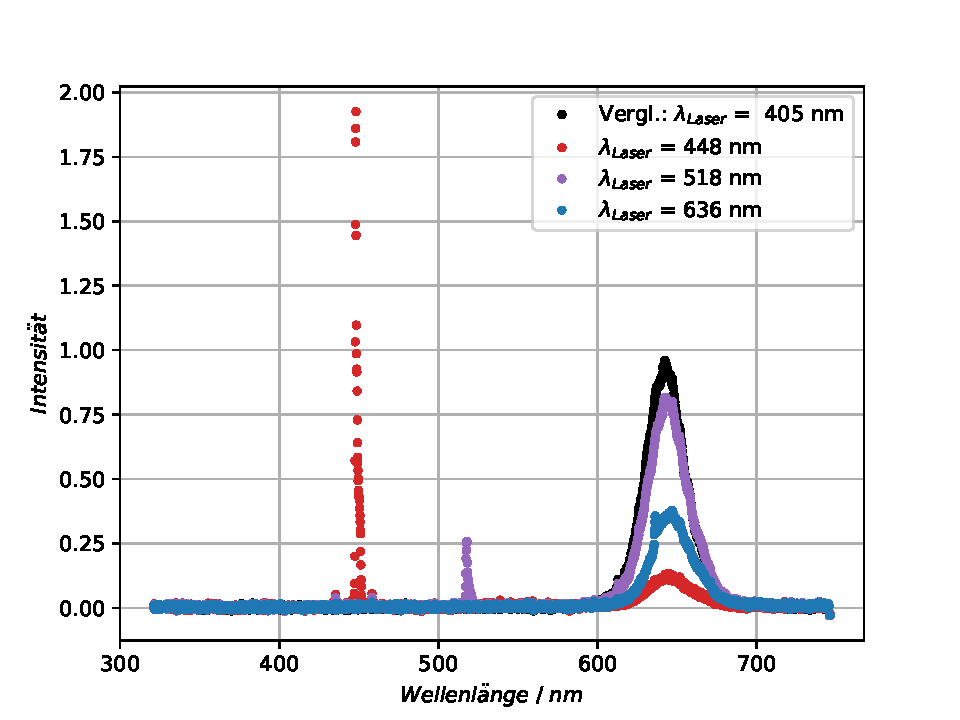
\includegraphics[width=\textwidth]{Plots/aufgabe2P1.pdf}
	\caption{PL-Spektren der Probe 1 mit unterschiedlicher Anregungswellenl\"{a}nge.}
	\label{}
	\end{subfigure}
	~
	\begin{subfigure}[t]{0.45\textwidth}
	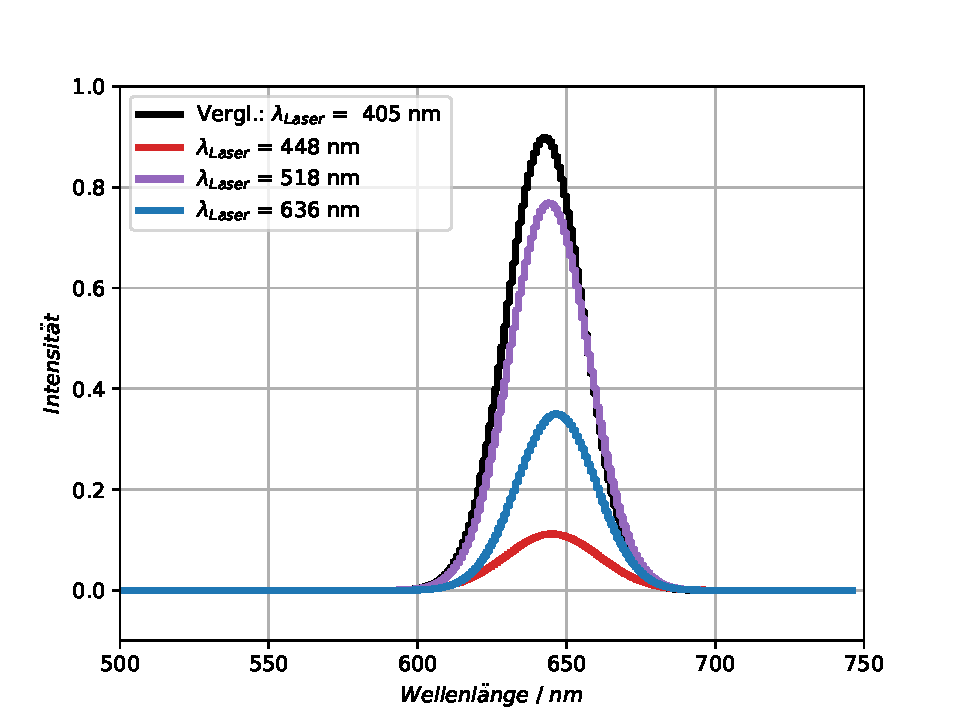
\includegraphics[width=\textwidth]{Plots/aufgabe2P1_fit_1s.pdf}
	\caption{Darstellung der Fits der Reflexionspeaks.}
	\label{}
	\end{subfigure}
\label{}
\end{figure}


\begin{figure}[hbtp]
\centering
\caption{Messungen und Ergebnisse zur Probe 2.}
	\begin{subfigure}[t]{0.45\textwidth}
	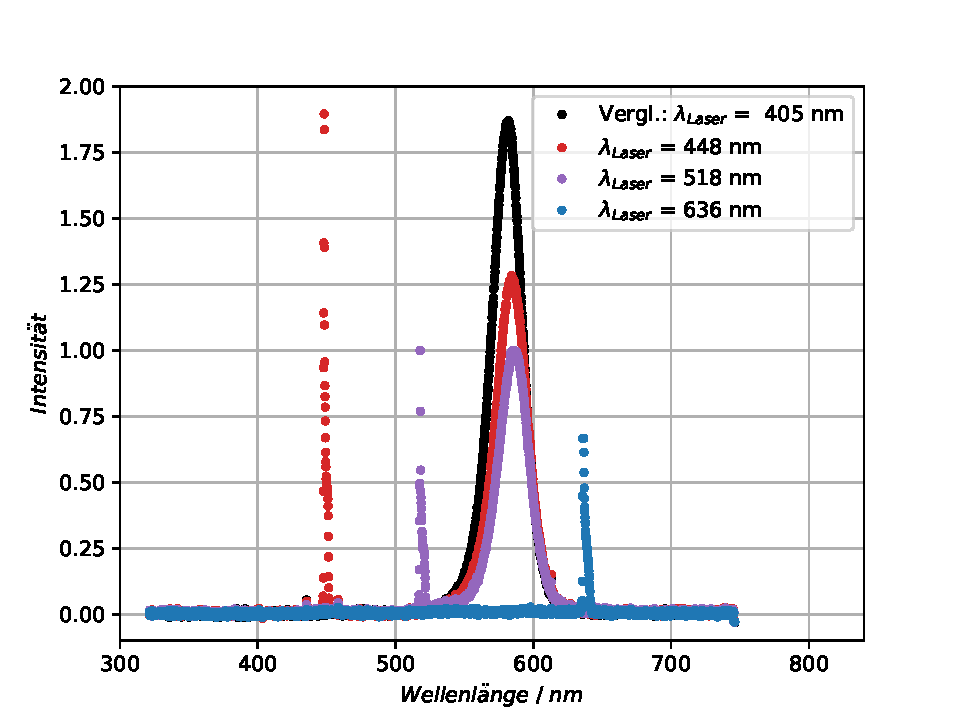
\includegraphics[width=\textwidth]{Plots/aufgabe2P2.pdf}
	\caption{PL-Spektren der Probe 2 mit unterschiedlicher Anregungswellenl\"{a}nge.}
	\label{}
	\end{subfigure}
	~
	\begin{subfigure}[t]{0.45\textwidth}
	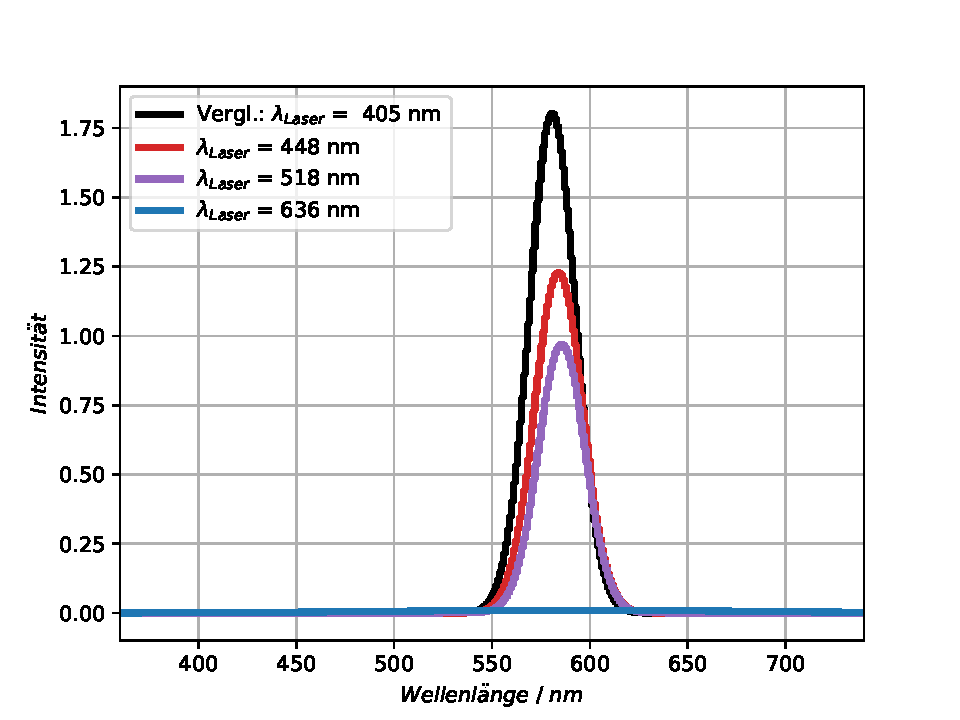
\includegraphics[width=\textwidth]{Plots/aufgabe2P2_fit_1s.pdf}
	\caption{Darstellung der Fits der Reflexionspeaks.}
	\label{}
	\end{subfigure}
\label{}
\end{figure}


\begin{figure}[hbtp]
\centering
\caption{Messungen und Ergebnisse zur Probe 3.}
	\begin{subfigure}[t]{0.45\textwidth}
	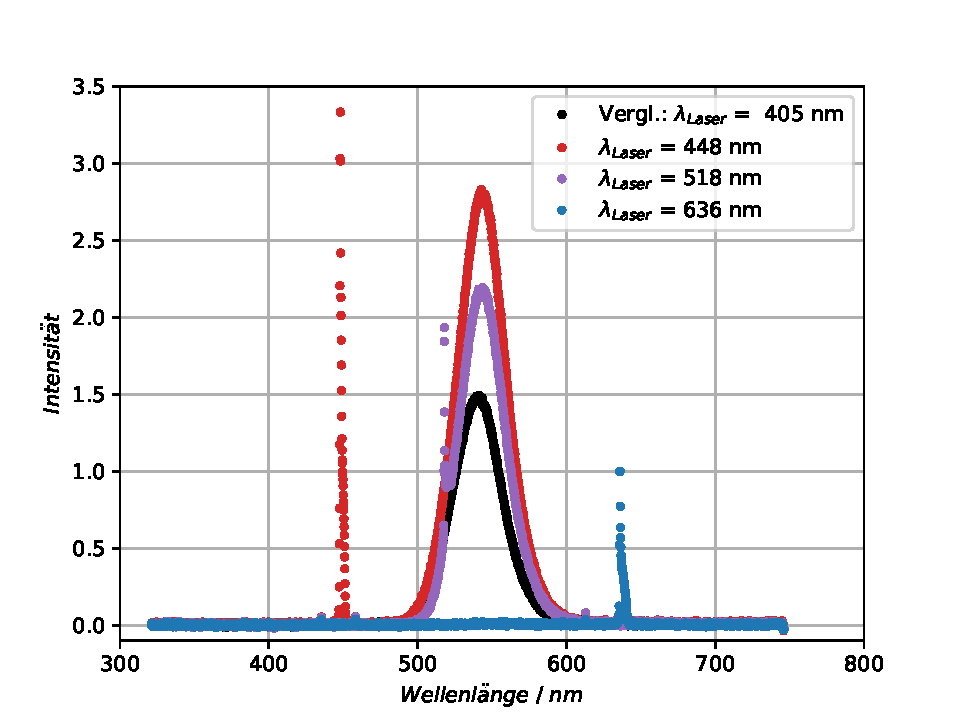
\includegraphics[width=\textwidth]{Plots/aufgabe2P3.pdf}
	\caption{PL-Spektren der Probe 3 mit unterschiedlicher Anregungswellenl\"{a}nge.}
	\label{}
	\end{subfigure}
	~
	\begin{subfigure}[t]{0.45\textwidth}
	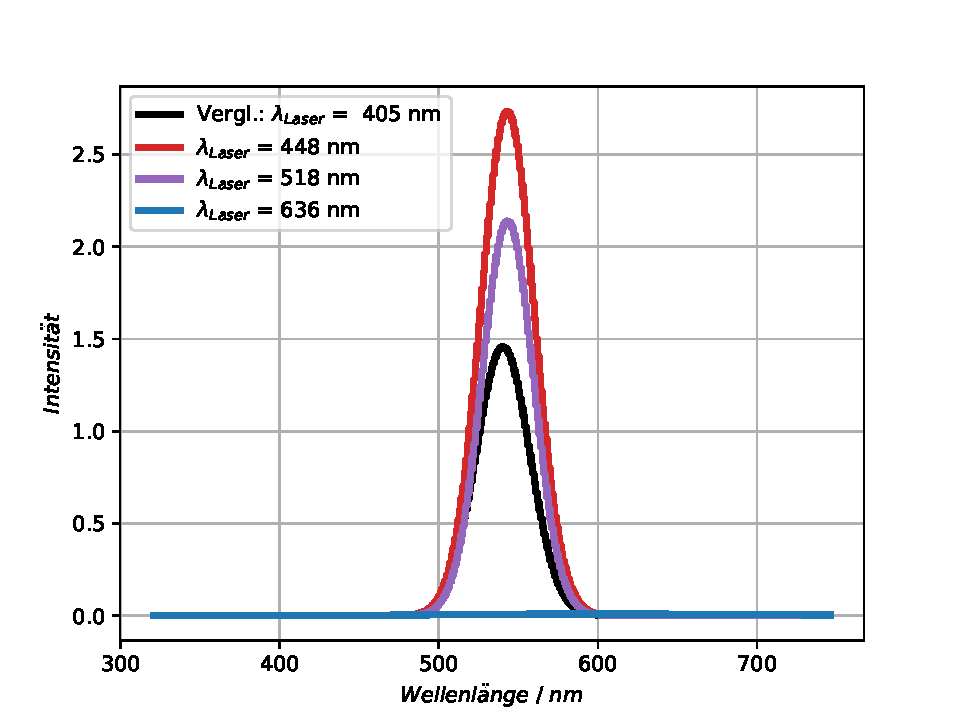
\includegraphics[width=\textwidth]{Plots/aufgabe2P3_fit_1s.pdf}
	\caption{Darstellung der Fits der Reflexionspeaks.}
	\label{}
	\end{subfigure}
\label{}
\end{figure}


\subsection{Linearer Polarisationsgrad von Flüssigkeiten (Bonus-Aufgabe)}

\begin{figure}[hbtp]
\centering
\caption{Die PL-Spektren der Messungen von der Wein-Probe f\"{u} verschiedene Polarisationspfade.}
	\begin{subfigure}[t]{0.45\textwidth}
	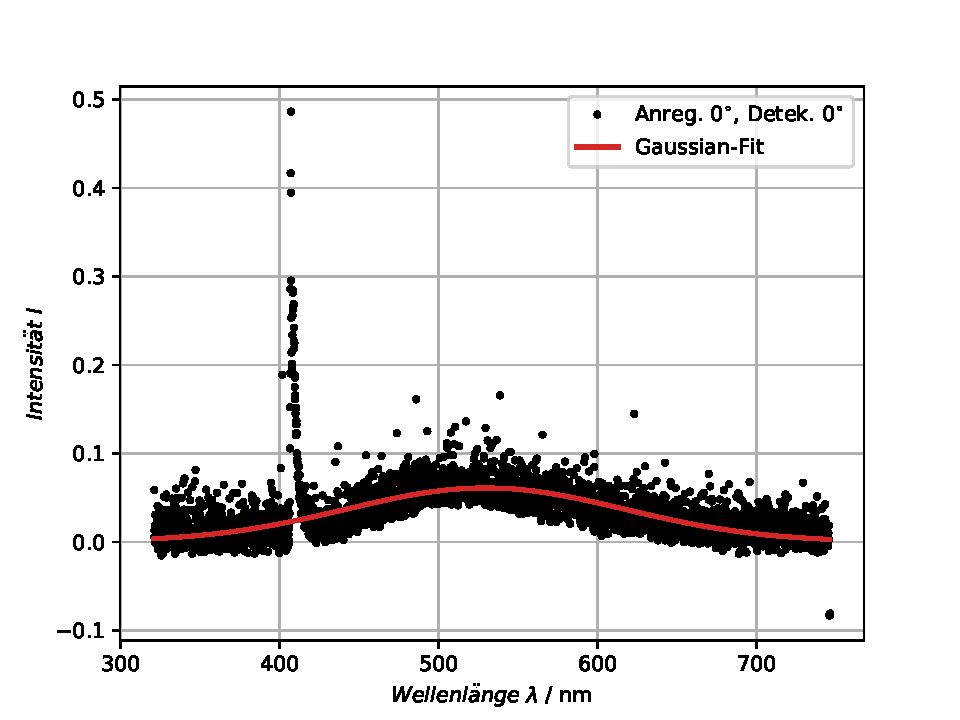
\includegraphics[width=\textwidth]{Plots/aufgabe3_P1.pdf}
	%\caption{}
	%\label{}
	\end{subfigure}
	%~
	\begin{subfigure}[t]{0.45\textwidth}
	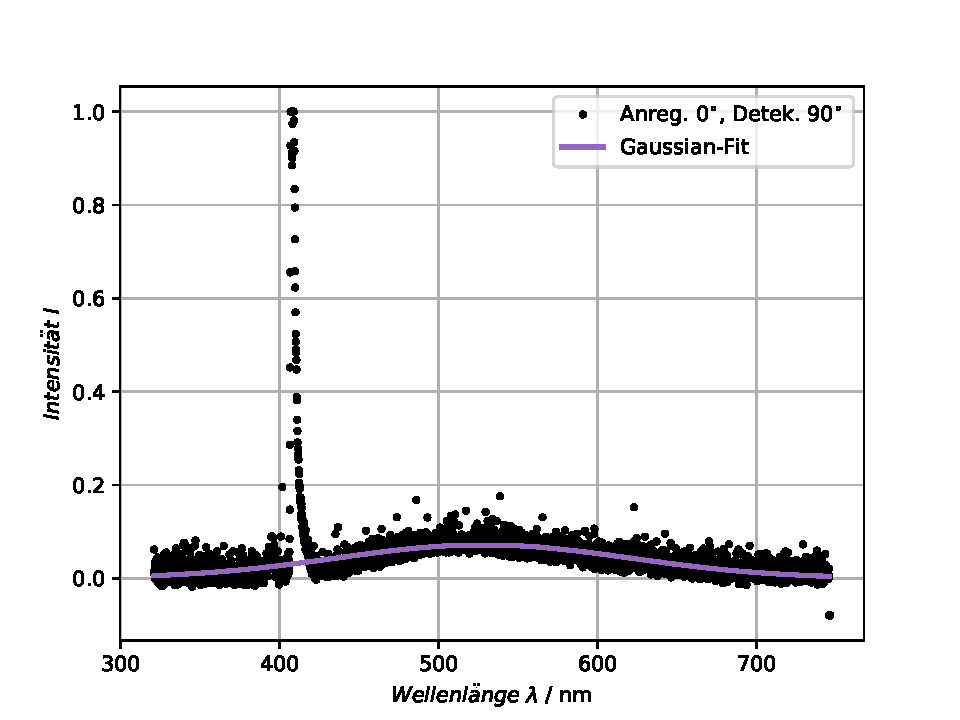
\includegraphics[width=\textwidth]{Plots/aufgabe3_P2.pdf}
	%\caption{.}
	%\label{}
	\end{subfigure}
	\\
	\begin{subfigure}[t]{0.45\textwidth}
	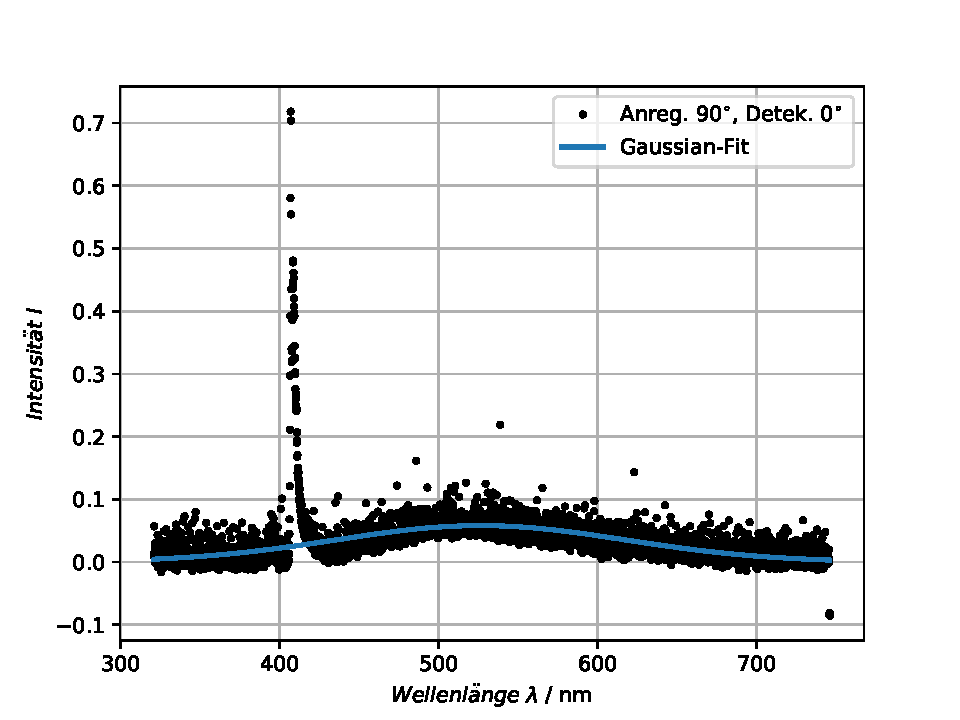
\includegraphics[width=\textwidth]{Plots/aufgabe3_P3.pdf}
	%\caption{}
	%\label{}
	\end{subfigure}
	%~
	\begin{subfigure}[t]{0.45\textwidth}
	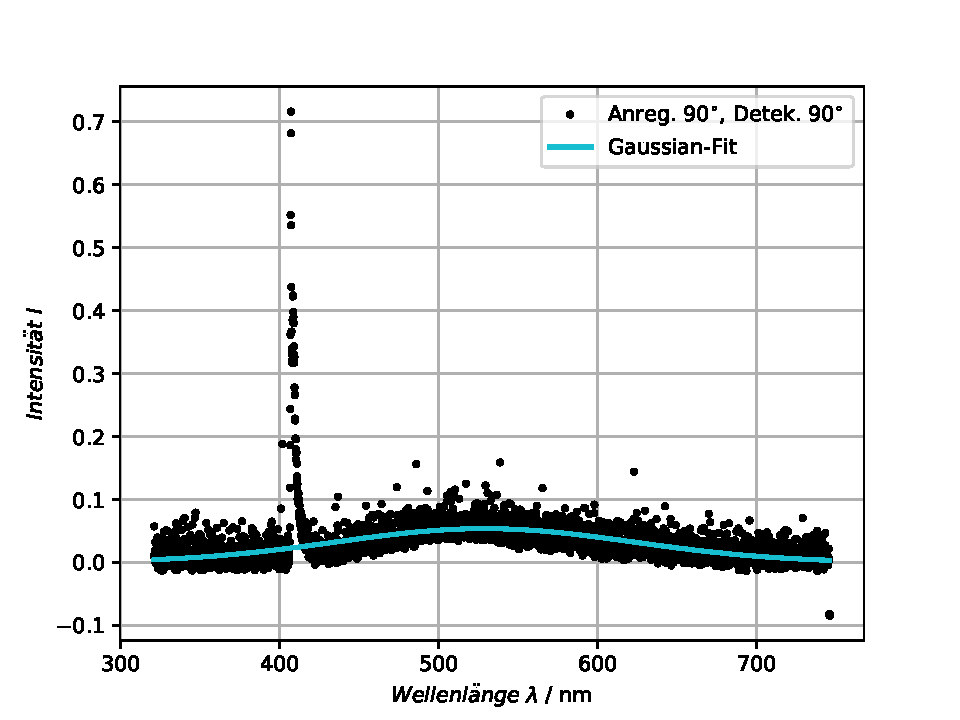
\includegraphics[width=\textwidth]{Plots/aufgabe3_P4.pdf}
	%\caption{.}
	%\label{}
	\end{subfigure}
\label{abb:auf3}
\end{figure}


\begin{figure}[hbtp]
\centering
\caption{Vergleich der vier Messung der Wein-Probe.}
	\begin{subfigure}{0.45\textwidth}
	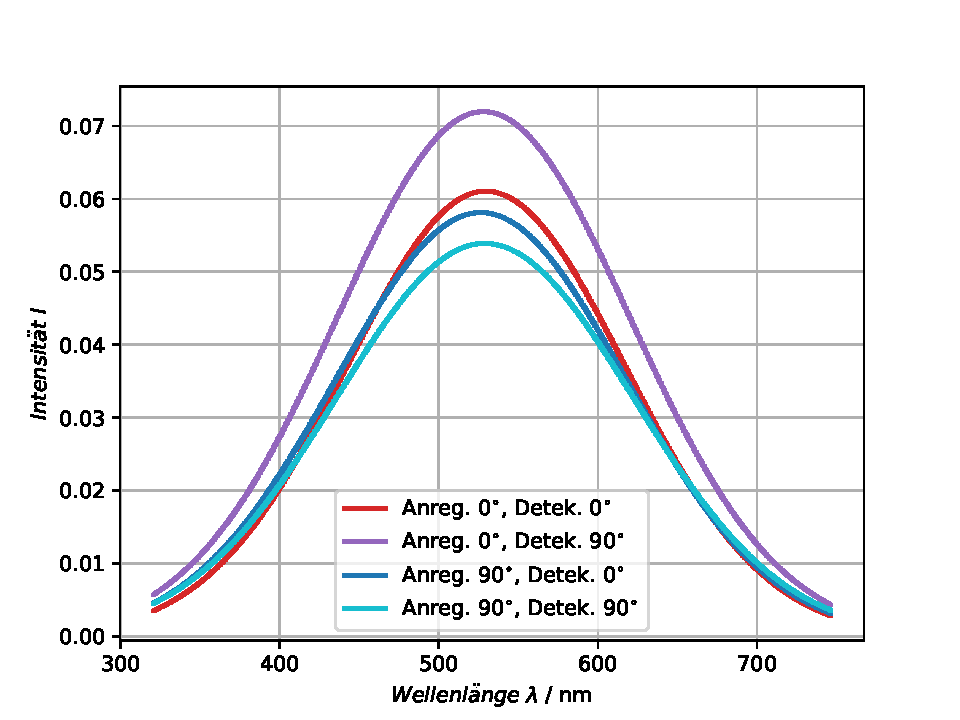
\includegraphics[width=\textwidth]{Plots/aufgabe3_vergleich.pdf}
	\caption{Die gefitteten Gau{\ss}-Kurven der vier gemessenen PL-Spektren im Vergleich.}
	\label{abb:auf3_vergleich}
	\end{subfigure}
	~
	\begin{subtable}{0.45\textwidth}
	\caption{Messwerte zu den gefitteten Gau{\ss}-Kurven.}
	\begin{tabular}{|rrc|}
	\hline
	{Anregung} & {Detektion} & {Intensit\"{a}tsmaximum} \\
	\hline
	$0^{\circ}$ & $0^{\circ}$ & 0,0611 \\
	$0^{\circ}$ & $90^{\circ}$ & 0,0719 \\
	$90^{\circ}$ & $0^{\circ}$ & 0,0581 \\
	$90^{\circ}$ & $90^{\circ}$ & 0,0539 \\
	\hline
	\end{tabular}
	\end{subtable}
\label{auf3}
\end{figure}


\begin{align}
	\text{Polarisationsgrad} = \frac{I_{PL,0^{\circ}} - I_{PL,90^{\circ}}}{I_{PL,0^{\circ}} + I_{PL,90^{\circ}}}
\end{align}

\begin{align*}
	\text{P}_{0^{\circ}} &= 0,08204 \\
	\text{P}_{90^{\circ}} &= 0,03779 \\	
\end{align*}